\begin{flushright} {\tiny {\color{gray} basis\_P1\_2D.tex}} \end{flushright}
%~~~~~~~~~~~~~~~~~~~~~~~~~~~~~~~~~~~~~~~~~~~~~~~~~~~~~~~~~~~~~~~~~~~~~~~~~~~~~~~~~~~~~~~~~~~~~~~~~~

Here we do not start from a reference element but consider instead a generic triangle:

\begin{flushright} {\tiny {\color{gray} (tikz\_P1.tex)}} \end{flushright}
%~~~~~~~~~~~~~~~~~~~~~~~~~~~~~~~~~~~~~~~~~~~~~~~~~~~~~~~~~~~~~~~~~~~~~~~~~~~~~~~~~~~~~~~~~~~~~~~~~~

\begin{center}
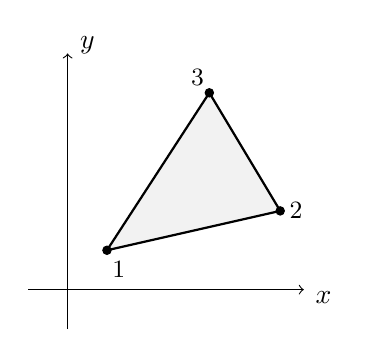
\begin{tikzpicture}
%\draw[step=0.5cm,gray,very thin] (0,0) grid (4,4); 
\draw[fill=gray!10,gray!10](1,1) (1,1)--(3.2,1.5)--(2.3,3)--cycle;
\draw[thick] (1,1)--(3.2,1.5)--(2.3,3)--cycle;
\draw [->] (0,0.5) -- (3.5,0.5);
\draw [->] (0.5,0) -- (0.5,3.5);
\node[] at (3.75,0.4) {$x$};
\node[] at (0.75,3.6) {$y$};
\draw[black,fill=black] (1,1)   circle (1.5pt);
\draw[black,fill=black] (3.2,1.5)   circle (1.5pt);
\draw[black,fill=black] (2.3,3)   circle (1.5pt);
\node[] at (1.15,0.75) {\small $1$};
\node[] at (3.4,1.5) {\small $2$};
\node[] at (2.15,3.2) {\small $3$};
\end{tikzpicture}
\end{center}




This is the simplest 2D element, which is also called linear triangular element.
Velocities (or displacements) $(u^h,v^h)$ in the element are interpolated from nodal velocities
$(u_i,v_i)$ using basis functions $\bN_i$ as follows,
\[
\left(
\begin{array}{c}
u^h(x,y) \\v^h(x,y)
\end{array}
\right)
=
\left(
\begin{array}{cccccc}
\bN_1(x,y) & 0 & \bN_2(x,y) & 0 & \bN_3(x,y) & 0\\
0 & \bN_1(x,y) & 0 & \bN_2(x,y) & 0 & \bN_3(x,y)\\
\end{array}
\right)
\cdot
\left(
\begin{array}{c}
u_1 \\ v_1 \\ u_2 \\ v_2 \\ u_3 \\ v_3
\end{array}
\right)
\]
or simply 
\[
u^h(x,y)=\sum_{i=1}^3 \bN_i(x,y) u_i
\qquad
\qquad
v^h(x,y)=\sum_{i=1}^3 \bN_i(x,y) v_i
\]

For this element, we have three nodes at the vertices of the triangle, which are 
numbered around the element in the counterclockwise direction. 
Each node has two degrees of freedom (can move in the $x$ and $y$ directions). 
The velocities $u^h$ and $v^h$ are assumed to be linear functions within the element, that is, 
\begin{eqnarray}
u^h(x,y)&=&b_1 +b_2x+b_3y \nn\\
v^h(x,y)&=&b_4 +b_5x+b_6y
\end{eqnarray}
where $b_i$ are constants to be determined and which depend on the triangle shape.
Note that the strain rate components are then given by
\begin{eqnarray}
\dot\varepsilon_{xx}&=&b_2  \nn\\
\dot\varepsilon_{yy}&=&b_6  \nn\\
\dot\varepsilon_{xy}&=&(b_3+b_5)/2 \nn
\end{eqnarray}
and are constant throughout the element.

The velocities should satisfy the following six equations:
\begin{eqnarray}
u_1 &=& u^h(x_1,y_1)= b_1 + b_2x_1+b_3y_1 \nn\\
u_2 &=& u^h(x_2,y_2)= b_1 + b_2x_2+b_3y_2 \nn\\
u_3 &=& u^h(x_3,y_3)= b_1 + b_2x_3+b_3y_3 \nn\\
v_1 &=& v^h(x_1,y_1)= b_4 + b_5x_1+b_6y_1 \nn\\
v_2 &=& v^h(x_2,y_2)= b_4 + b_5x_2+b_6y_2 \nn\\
v_3 &=& v^h(x_3,y_3)= b_4 + b_5x_3+b_6y_3 \nn
\end{eqnarray}
Let us focus on the three equations with the $u$ component of the velocity.
These can be re-written:
\[
\left(
\begin{array}{c}
u_1 \\ u_2 \\ u_3  
\end{array}
\right)
=
\left(
\begin{array}{ccc}
1 & x_1 & y_1 \\
1 & x_2 & y_2 \\
1 & x_3 & y_3 \\
\end{array}
\right)
\cdot
\left(
\begin{array}{c}
b_1 \\ b_2 \\ b_3  
\end{array}
\right)
\]
In order to obtain $b_1,b_2,b_3$ we need to solve this system, or simply to compute the
inverse of the $3\times 3$ ${\bm M}$ matrix, as explained in Appendix~\ref{sec:inv3x3}.

We define $D={\rm det}({\bm M})$ and we get
\[
\left(
\begin{array}{c}
b_1 \\ b_2 \\ b_3  
\end{array}
\right)
=
\frac{1}{D}
\tilde{\bm M}
\cdot
\left(
\begin{array}{c}
u_1 \\ u_2 \\ u_3  
\end{array}
\right)
%\qquad
%{\rm and}
%\qquad
%\left(
%\begin{array}{c}
%b_4 \\ b_5 \\ b_6  
%\end{array}
%\right)
%=
%\frac{1}{D}
%\tilde{\bm M}
%\cdot
%\left(
%\begin{array}{c}
%v_1 \\ v_2 \\ v_3  
%\end{array}
%\right)
\]
The matrix $\tilde{\bm M}$ writes:
\[
\tilde{\bm M}
%=
%\left(
%\begin{array}{ccc}
%  x_2y_3-x_3y_2  & -(y_3-y_2) &   x_3-x_2 \\
%-(x_1y_3-x_3y_1) &   y_3-y_1  & -(x_3-x_1) \\
%  x_1y_2-x_2y_1  & -(y_2-y_1) &   x_2-x_1
%\end{array}
%\right)
=
\left(
\begin{array}{ccc}
x_2y_3-x_3y_2 & x_3y_1-x_1y_3 & x_1y_2-x_2y_1 \\
y_2-y_3 & y_3-y_1  & y_1-y_2 \\
x_3-x_2 & x_1-x_3 & x_2-x_1 
\end{array}
\right)
\]
so that 
\begin{eqnarray}
b_1 &=& \frac1D [ (x_2y_3-x_3y_2)u_1 + (x_3y_1-x_1y_3)u_2 + (x_1y_2-x_2y_1)u_3 ] \nn\\
b_2 &=& \frac1D [ (y_2-y_3)u_1 + (y_3-y_1)u_2 + (y_1-y_2)u_3 ] \nn\\
b_3 &=& \frac1D [ (x_3-x_2)u_1 + (x_1-x_3)u_2 + (x_2-x_1)u_3 ]
\end{eqnarray}
We then have
\begin{eqnarray}
u^h(x,y) 
&=& b_1 + b_2 x + b_3 y \nn\\
&=&\frac1D [(x_2y_3-x_3y_2)u_1 + (x_3y_1-x_1y_3)u_2 + (x_1y_2-x_2y_1)u_3 ] \nn\\
&+&\frac1D [(y_2-y_3)u_1 + (y_3-y_1)u_2 + (y_1-y_2)u_3]x \nn\\
&+&\frac1D [(x_3-x_2)u_1 + (x_1-x_3)u_2 + (x_2-x_1)u_3]y \nn\\
&=&\frac1D [(x_2y_3-x_3y_2) + (y_2-y_3)x + (x_3-x_2)y]u_1\nn\\ 
&+&\frac1D [(x_3y_1-x_1y_3) + (y_3-y_1) x + (x_1-x_3) y]u_2 \nn\\
&+&\frac1D [(x_1y_2-x_2y_1) + (y_1-y_2) x + (x_2-x_1) y]u_3\nn\\
&=& \bN_1(x,y) u_1 + \bN_2(x,y) u_2 + \bN_3(x,y) u_3
\end{eqnarray}
with the linear basis functions are given by:
\begin{eqnarray}
\bN_1(x,y) &=& \frac{1}{D}[(x_2y_3-x_3y_2) + (y_2-y_3)x + (x_3-x_2)y] \nn\\
\bN_2(x,y) &=& \frac{1}{D}[(x_3y_1-x_1y_3) + (y_3-y_1)x + (x_1-x_3)y] \nn\\
\bN_3(x,y) &=& \frac{1}{D}[(x_1y_2-x_2y_1) + (y_1-y_2)x + (x_2-x_1)y] \nn
\end{eqnarray}
Importantly we can easily verify that for example
\[
\bN_2(x_1,y_1)= \frac{1}{D}[(x_3y_1-x_1y_3) + (y_3-y_1)x_1 + (x_1-x_3)y_1] = 0
\]
\[
\bN_2(x_2,y_2)= \frac{1}{D}[(x_3y_1-x_1y_3) + (y_3-y_1)x_2 + (x_1-x_3)y_2] = 1
\]
Note that the area $A$ of the triangle is given by:
\[
A=\frac{1}{2}D = \frac{1}{2}
\left|
\begin{array}{ccc}
1 & x_1 & y_1 \\
1 & x_2 & y_2 \\
1 & x_3 & y_3 
\end{array}
\right|
\]

\noindent If we now consider the reference element in the reduced coordinates space $(r,s)$:

\begin{flushright} {\tiny {\color{gray} (tikz\_P1ref.tex)}} \end{flushright}
%~~~~~~~~~~~~~~~~~~~~~~~~~~~~~~~~~~~~~~~~~~~~~~~~~~~~~~~~~~~~~~~~~~~~~~~~~~~~~~~~~~~~~~~~~~~~~~~~~~


\begin{center}
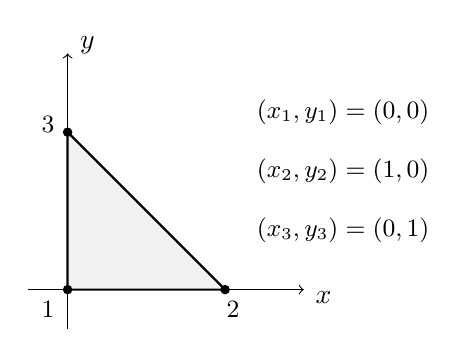
\begin{tikzpicture}
%\draw[step=0.5cm,gray,very thin] (0,0) grid (4,4); 
\draw[fill=gray!10,gray!10] (0.5,0.5)--(2.5,0.5)--(0.5,2.5)--cycle;
\draw[thick] (0.5,0.5)--(2.5,0.5)--(0.5,2.5)--cycle;
\draw [->] (0,0.5) -- (3.5,0.5);
\draw [->] (0.5,0) -- (0.5,3.5);
\node[] at (3.75,0.4) {$x$};
\node[] at (0.75,3.6) {$y$};
\draw[black,fill=black] (0.5,0.5)   circle (1.5pt);
\draw[black,fill=black] (2.5,0.5)   circle (1.5pt);
\draw[black,fill=black] (0.5,2.5)   circle (1.5pt);
\node[] at (0.25,0.25) {\small $1$};
\node[] at (2.6,0.25) {\small $2$};
\node[] at (0.25,2.6) {\small $3$};
\node[] at (4,2.75) {\small $(x_1,y_1)=(0,0)$};
\node[] at (4,2) {\small $(x_2,y_2)=(1,0)$};
\node[] at (4,1.25) {\small $(x_3,y_3)=(0,1)$};
\end{tikzpicture}
\end{center}



The basis polynomial is then
\[
f(r,s) = a + br + cs 
\]
and the basis functions:
\begin{mdframed}[backgroundcolor=blue!5]
\begin{eqnarray}
\bN_0(r,s) &=& 1-r-s \\
\bN_1(r,s) &=& r \\
\bN_2(r,s) &=& s 
\end{eqnarray}
\end{mdframed}
Once again we can verify that $\bN_i(x_j,y_j)=\delta_{ij}$ and $\sum_i \bN_i(r,s)=1$.



